
% vim:set ff=unix expandtab ts=2 sw=2:
%%%%%%%%%%%%%%%%%%%%%%%%%%%%%%%%%%%%%%%%%%%%%%%%%%%%%%%%%%%%%%%%%%%%%%%%%%%%%%
%%% Here starts the poster
%%%---------------------------------------------------------------------------
%%% Format it to your taste with the options
%%%%%%%%%%%%%%%%%%%%%%%%%%%%%%%%%%%%%%%%%%%%%%%%%%%%%%%%%%%%%%%%%%%%%%%%%%%%%%
% Define some colors

\definecolor{lightblue}{rgb}{.187,.613,.594}
%\definecolor{lightblue}{rgb}{0.145,0.6666,1}


\hyphenation{resolution occlusions}
%%
\newcommand{\numberofcolumns}{5}
%  % we set some new variables
  \newcommand{\leftspan}{2}
  \newcommand{\leftcol}{1}

\begin{tcbposter}[
  poster = {
    %showframe,
    height=\the\dimexpr \textheight-\footsep * 2 \relax,
    %height=\textheight,
    spacing=\footsep,
    columns = \numberofcolumns,
  },
  boxes = {
    beamer,
    colframe=lightgray,
    %colbacktitle=red!50!white,
    colbacktitle=lightgray,
    coltitle=darkgray,
    %colframe=blue!50!black,
    %colback=blue!50,
    colback=lightgray,
    colupper=black!50,
    coltext=black
    %fonttitle=\bfseries\Large\scshape
  },
  fontsize =29.5pt
]
%  %%%---------------------------------------------------------------------------

  \edef\rightspan{\the\numexpr (\numberofcolumns - \leftspan) \relax}
  \edef\rightcol{\the\numexpr \leftspan+\leftcol\relax} 
  %%%%%%%%%%%%%%%%%%%%%%%%%%%%%%%%%%%%%%%%%%%%%%%%%%%%%%%%%%%%%%%%%%%%%%%%%%%%%%
  % first column  
    % top
  \posterbox[ title =Challenge]{
      name=Challenge,
      span=\leftspan,
      column=\leftcol, 
    }{
	  	
% vim:set ff=unix expandtab ts=2 sw=2:
\noindent
Many models in ecology and biogeochemistry, in particular models of the global
carbon cycle, can be generalized as systems of non-autonomous ordinary
differential equations (ODEs). For many applications, it is important to
determine the stability properties for this type of systems, but most methods
available for autonomous systems are not necessarily applicable for the
non-autonomous case.  We discuss here stability notions for non-autonomous
nonlinear models represented by systems of ODEs explicitly dependent on time
and a time-varying input signal.  
Is there a stability concept that is:
\begin{enumerate}
	\item
	broad enough to encompass these models
	\item
	rigorous enough to be proved analytically 
	\item
	interpretable in ecologically meaningful terms ?
\end{enumerate}

    %\the\rightspan
	  }
    %%%%%%%%%%%%%%%%%%%%%%%%%%%%%%%%%%%%%%%%%%%%%%%%%%%%%%%%%%%%%%%%%%%%%%%%%%%%%%
    % bottom 
    \posterbox[title = {Results I, ISS as generalization of available stability concepts}]{
      name=generalsoilmodel,
      span=\leftspan,
      column=\leftcol, 
      above=bottom
    }{
	  	
% vim:set ff=unix expandtab ts=2 sw=2:
%\begin{multicols}{2}
\begin{center}
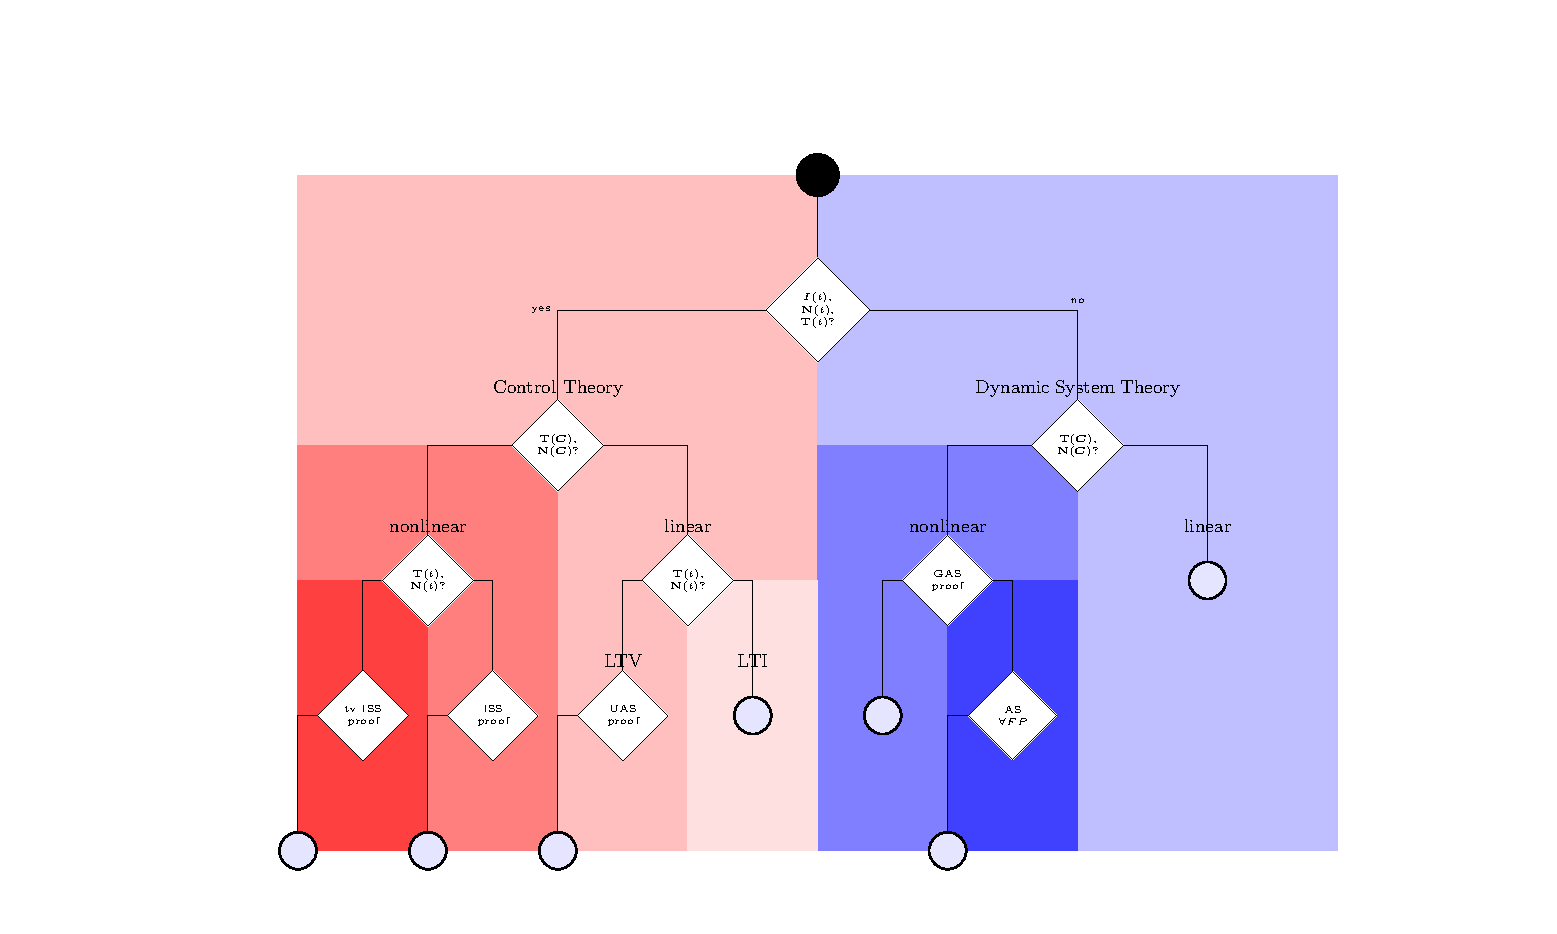
\includegraphics[width=\columnwidth,clip=true,trim=4.5cm 1cm 3.2cm 2cm]{Fig1.pdf}
\end{center}

%\columnbreak
\noindent
The graph shows different stability concepts one could try to establish for the
general soil model mentioned above depending on properties of its components 
$\mathbf{I},\mathbf{T}$ and $ \mathbf{N}$. The hardest to prove is Input to
State Stability for time varying systems (ISStv) in the lower left corner.  It
turns out that ISStv also generalizes all the other concepts mentioned:
\begin{itemize}
\item 
In the case of Linear Time Invariant (LTI) systems  ISS follows from the properties of the matrix.(eigenvalues)
\item 
In the case of Linear Time Variant (LTV) systems it can be established if sufficient information about the 
state transition operator allows to prove uniform asymptotic stability UAS.
\item
For input free system (on the blue right-hand side) ISS reduces to Global Asymptotic Stability (GAS)
\item
\dots

\end{itemize}
%\end{multicols}

	  }
	  %%%%%%%%%%%%%%%%%%%%%%%%%%%%%%%%%%%%%%%%%%%%%%%%%%%%%%%%%%%%%%%%%%%%%%%%%%%%%%
    % middle
    \posterbox[title={ Example: general soil model }]{
      name=general,
      span=\leftspan,
      column=\leftcol,
      between=Challenge and generalsoilmodel
    }{
	  	
% vim:set ff=unix expandtab ts=2 sw=2:
\centering
\begin{multicols}{2}
    		\[
		\mathbf{\dot{C}}= \bm{I}(t) + {\bf T}(\mathbf{C},t) \cdot {\bf N}(t, \bm{C}) \cdot \bm{C}(t)
    		\]
    		\begin{equation*}	
    		\label{structCond}
    		\begin{array}{lcl}	
    		N_{i,i}(\mathbf{C},t) 		&\ge& 	 0 \quad \forall i \\
    		T_{i,i}(\mathbf{C},t) 		&=& 	 -1 \quad \forall i \\
    		T_{i,j}(\mathbf{C},t) 		&\ge& 	 0 \quad \forall i \ne j \\
    		\sum_i T_{i,j}(\mathbf{C},t) 	&=  &	 1\quad \forall j 
    		\end{array}	
    		\end{equation*}	
    		This model structure generalizes most SOM decomposition models with any arbitrary number of pools, including those describing nonlinear interactions among state variables. It enforces mass balance and substrate dependence of decomposition, and it is flexible enough to describe:
		\begin{enumerate}
		\item Heterogeneity of decomposition rates
		\item Transformations of organic matter
		\item Environmental variability effects
		\item Organic matter interactions
		\end{enumerate}

		Examples for nonlinear models are:
		\begin{enumerate}
			\item Exoenzyme models \citep{Schimel,Sinsabaugh}
			\item AWB \citep{Allison}
			\item Bacwave \citep{Zelenev}
			\item MEND \citep{WangMEND}
			\item Manzoni \citep{Manzoni07}
		\end{enumerate}
		Also linear models fit into the general framework 
		\begin{enumerate}
			\item Henin's model \citep{HeninDupuis, Henin}
			\item ICBM \citep{AndrenKatterer}
			\item RothC \citep{Jenkinson, Coleman} 
			\item Century \citep{Parton} 
			\item Fontaine 1-4 \citep{Fontaine}
		\end{enumerate}
\end{multicols}
One general concept to encompass especially  these nonlinear  models is clearly desirable.

	  }
  %%%%%%%%%%%%%%%%%%%%%%%%%%%%%%%%%%%%%%%%%%%%%%%%%%%%%%%%%%%%%%%%%%%%%%%%%%%%%%
  % second column  
    % top
      \posterbox[title= {Results II, ISS like behavior and proof for example system }]{
        name=combi, 
        column=\rightcol, 
        span= \rightspan
      }{
    	  
% vim:set ff=unix expandtab ts=2 sw=2:
%\begin{columns}
%  \newlength{\lc}
%  \setlength{\lc}{0.4\textwidth}
%  \newlength{\rc}
%  \setlength{\rc}{\dimexpr(\textwidth-\lc) \relax}
%  \begin{column}{\lc}
\begin{multicols}{2}
  The graphs show the reactions of a prototypical class of nonlinear two pool soil models to a disturbing time varying signal. 
  This model is a technically simple place holder for ecologically motivated nonlinear systems like the soil models mentioned above to be analyzed in the future. It is given by:\\
  \begin{eqnarray*}
  \dot{C}_x=I_{x}(t)  - \left(C_{x}^{2} + C_{x}\right) \operatorname{k_{x}}{\left (t \right )}\\
  \dot{C}_y=I_{y}(t)  - \left(C_{y}^{2} + C_{y}\right) \operatorname{k_{y}}{\left (t \right )}
  \end{eqnarray*}
  where $C_x,C_y$ are the carbon contents of two unconnected pools and the bounded  periodic functions $k_x(t) $ and $k_y(t) $ with:\\ 
  \begin{eqnarray*}
  k_{x_{min}}\le  k_x(t) \le k_{x_{max}} \\k_{y_{min}} \le  k_y(t) \le k_{y_{max}}
  \end{eqnarray*}
  describe the seasonal changes in decomposition speed.
  e.g.:\\ 
  \begin{eqnarray*}
  k_x=\frac{k_{xmax}}{2} + \frac{k_{xmin}}{2} + \frac{1}{2} \left(k_{xmax} - k_{xmin}\right) \sin{\left (4 t \right )}\\k_y=\frac{k_{ymax}}{2} + \frac{k_{ymin}}{2} + \frac{1}{2} \left(k_{ymax} - k_{ymin}\right) \sin{\left (4 t \right )}
  \end{eqnarray*}
  The system can have a fixed point: 
  $$ \mathbf{C}_f= \begin{pmatrix} C_{fx} \\ C_{fy} \end{pmatrix} $$
  if the input streams have the same period and phase as the decomposition rates. For constant input streams it stays in a predictable region (an invariant set in the phase plane) \\ 
  \begin{eqnarray*}
  \mathbf{I}_0(t)=\left(
      \begin{pmatrix}
        \left( C_{fx}^{2} + C_{fx} \right) \operatorname{k_{x}}{\left (t \right )}\\
        \left( C_{fy}^{2} + C_{fy} \right)  \operatorname{k_{y}}{\left (t \right )}
      \end{pmatrix}
    \right)
  \end{eqnarray*}
  The fixpoint would be.
  \[
  \mathcal{A}=\{\mathbf{C}_f\}
  \]
  We will now disturb both mass influxes individually by perturbations $u_x(t),u_y(t)$ and get: 
  \begin{eqnarray*}
  \dot{C}_x=I_{0 x}(t) + u_{x}(t) - \left(C_{x}^{2} + C_{x}\right) \operatorname{k_{x}}{\left (t \right )}\\
  \dot{C}_y=I_{0 y}(t) + u_{y}(t) - \left(C_{y}^{2} + C_{y}\right) \operatorname{k_{y}}{\left (t \right )}
  \end{eqnarray*}
  The plots show the typical behavior of an ISS system: The changes in the state variables will asymptotically converge to a region of stability around an invariant set, whose size is a monotone function of the size of the disturbance (denoted by $|u|_{\infty}$).
  For this particular system we proved the ISS property rigorously. The proof relies on the construction of an ISS Lyapunov function whose choice is \emph{not determined but  inspired} by a property of the system interpretable in ecologically terms. Expressed casually: "The  system can counteract supply changes fast enough".
  This situation seems to be typical: The problem of establishing ISS for e.g. all the $\mathbf{I},\mathbf{T},\mathbf{N}$ models based on the ecologic principles they follow , is too hard.
  But bio-chemical of biophysical restrictions could provide clues to ISS proofs for a particular system.
  
%  \end{column}
%  \begin{column}{\rc}
    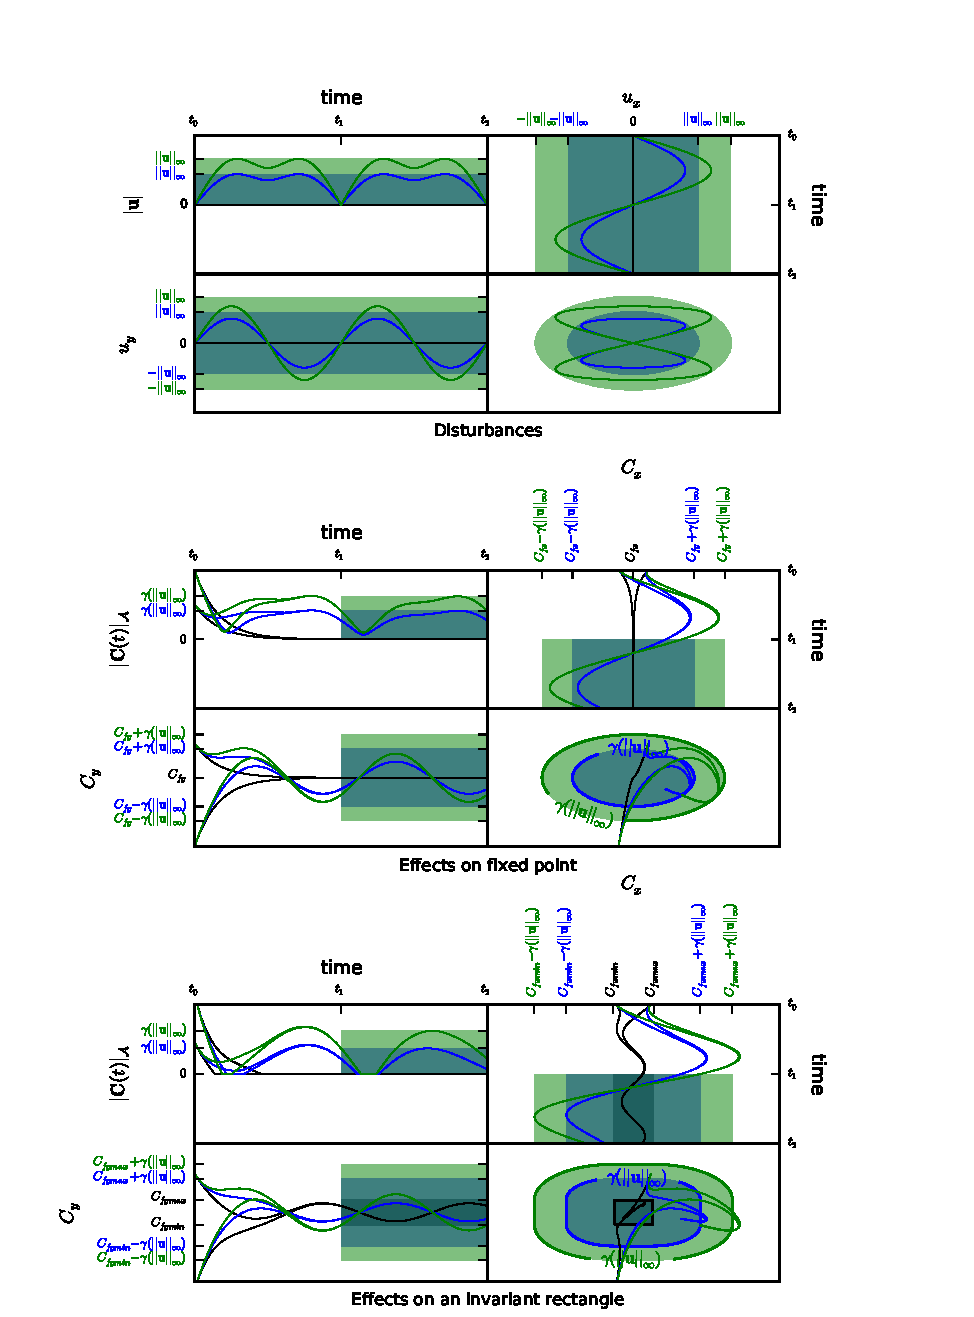
\includegraphics[width=\columnwidth,clip=true,trim=1.0cm 0cm 2cm 1cm]{combiPlot2.pdf}
    \begin{enumerate}
    	\item
    	The four plots on the top show the disturbances.
    	\item
    	The next four plots in the middle show the effect of this disturbances on the solutions for a system with fixed point. 
    	\item
    	The next four plots in the middle show the effect of this disturbances on the solutions for the system which no longer has a fixed point, but at least an invariant set, the dark blue square in the middle.
    \end{enumerate}
 % \end{column}
%\end{columns}
\end{multicols}
\vspace{1cm}

      }
    %%%%%%%%%%%%%%%%%%%%%%%%%%%%%%%%%%%%%%%%%%%%%%%%%%%%%%%%%%%%%%%%%%%%%%%%%%%%%%
    % bottom 
    \posterbox[title=Bibliography] {
      name=bibliography,
      span=\rightspan,
      column=\rightcol, 
      above=bottom
    }{
      {
        \tiny
       % \small
        \begin{multicols}{3}
          %\nobibliography{GeneralModel} % the citations are there but no Referenc section
          \renewcommand{\section}[2]{}% to get rid of the References Header
        %  
% vim:set ff=unix expandtab ts=2 sw=2:
\documentclass[final,hyperref={pdfpagelabels=false}, professionalmath, mathserif, 11pt]{beamer}
\mode<presentation>{\usetheme{SAB_2018}}

% There are many packages already loaded by beamerthemeBGC_retreat.sty
% put them in a file and load them here
  %
% vim:set ff=unix expandtab ts=2 sw=2:
\usepackage{caption}
\usepackage{subfigure}
\usepackage[utf8]{inputenc}
\usepackage[english]{babel}

  
% vim:set ff=unix expandtab ts=2 sw=2:
\usepackage{caption}
\usepackage{subfigure}
\usepackage{verbatim}
\usepackage{minted}
\usepackage[utf8]{inputenc}
\usepackage[english]{babel}
\usepackage[most,poster]{tcolorbox}


%%%%%%%%%%%%%%%%%%%%%%%%%%%%%%%%%%%%%%%%%%%%%%%%%%%%%%%%%%%%%%%%%%%%%%%%%%%%%%%%%%%%%
% obligatory macros expected by the style file
% You have to provide defintions here, since the template expects them

  % \myTitle
  \newcommand\myTitle{Application of Input to State Stability to ecological reservoir models}
  
  % \myDepartment 
  \newcommand\myDepartment{Department Biogeochemical Processes \vspace{1cm}}
  
  % \myFooter 
  % The macro has to be defined in input file
  
% vim:set ff=unix expandtab ts=2 sw=2:
\newlength{\pictureHeight}
\setlength{\pictureHeight}{3cm}

\newcommand{\peoplebox}[2]{
  \begin{minipage}[t]{3\pictureHeight}
    \centering{
    	\includegraphics[height=\pictureHeight]{#1}\\
	#2
    }
    \vspace{2cm}
  \end{minipage}
}

\newcommand{\logobox}[1]{\peoplebox{#1}{}}

%\def\myFooter{
\newcommand{\myFooter}{
  \logobox{images/logos/Minerva_green_text_en.pdf}
	\hfill
  \logobox{images/logos/EmmyNoether.jpg}
	\hfill
  \logobox{images/logos/IMPRS_Logo__skalierbar.pdf}
	\hfill
  \peoplebox{images/people/Metzler.jpg}{Holger Metzler}
	\hfill
  \peoplebox{images/people/MarkusMueller.jpg}{Markus Müller}
	\hfill
  \peoplebox{images/people/Sierra.jpg}{Carlos Sierra}
	\hfill
  \logobox{images/qrcode.png}
}
	
  % p.s.: We could define the macro here by the content of an input file
  % \newcommand{\myFooter}{
  %   \input{footerContent}
  % }
  % but then footerContent.tex could not contain any macro definitions,
  % since you would define a macro inside a macro...
  % and you would be forced to put your macros in a separate file to be sourced
  % earlier.
  % For the exmaples we wanted to keep the macros only needed in the 
  % footer to stay there.


\begin{document}
  \begin{frame}
  \vspace{3ex}

    %%%%%%%%%%%%%%%%%%%%%%%%%%%%%%%%%%%%%%%%%%%%%%%%%%%%%%%%%%%%%%%%%%%%%%%%%%%%%%%
    % main content
    
% vim:set ff=unix expandtab ts=2 sw=2:
%%%%%%%%%%%%%%%%%%%%%%%%%%%%%%%%%%%%%%%%%%%%%%%%%%%%%%%%%%%%%%%%%%%%%%%%%%%%%%
%%% Here starts the poster
%%%---------------------------------------------------------------------------
%%% Format it to your taste with the options
%%%%%%%%%%%%%%%%%%%%%%%%%%%%%%%%%%%%%%%%%%%%%%%%%%%%%%%%%%%%%%%%%%%%%%%%%%%%%%
% Define some colors

\definecolor{lightblue}{rgb}{.187,.613,.594}
%\definecolor{lightblue}{rgb}{0.145,0.6666,1}


\hyphenation{resolution occlusions}
%%
\newcommand{\numberofcolumns}{5}

\begin{tcbposter}[
  poster = {
    %showframe,
    height=\the\dimexpr \textheight-\footsep * 2 \relax,
    %height=\textheight,
    spacing=\footsep,
    columns = \numberofcolumns,
  },
  boxes = {
    beamer,
    colframe=lightgray,
    %colbacktitle=red!50!white,
    colbacktitle=lightgray,
    coltitle=darkgray,
    %colframe=blue!50!black,
    %colback=blue!50,
    colback=lightgray,
    colupper=black!50,
    coltext=black,
    %fonttitle=\bfseries\large\scshape
    fonttitle=\bfseries\Large\scshape
  },
  fontsize =29pt
]
%  %%%---------------------------------------------------------------------------
%  % we set some new variables
  \newcommand{\leftspan}{2}
  \newcommand{\leftcol}{1}

  \edef\rightspan{\the\numexpr (\numberofcolumns - \leftspan) \relax}
  \edef\rightcol{\the\numexpr \leftspan+\leftcol\relax} 
  %%%%%%%%%%%%%%%%%%%%%%%%%%%%%%%%%%%%%%%%%%%%%%%%%%%%%%%%%%%%%%%%%%%%%%%%%%%%%%
  % first column  
    % top
  \posterbox[ title =Overview]{
      name=Overview,
      span=\leftspan,
      column=\leftcol, 
    }{
	  	\begin{minipage}{\textwidth}
We find general formulas for the transit time and age distributions in well-mixed compartmental systems.
As an example we consider a simple three-pool global carbon model
 with nonlinearities in two different scenarios:
\end{minipage}

\begin{tabular}{rl}
\textbf{steady state} & pre-industrial system before 1765 \\
\textbf{perturbed} & adding fossil fuels to the atmosphere,\\
& considering land use change,\\
& 1765-2500
\end{tabular}

{\Large Main quantities of interest}

\begin{minipage}{\textwidth}
	\begin{tabular}{rl}
	 \textbf{transit time} & time that a particle needs to travel through\\
	 & the system\\
	 & exit time $-$ entry time\\
	 \textbf{system age} & for particles in the system\\
	 & current time $-$ entry time\\
	\textbf{compartment} & system age of particles in a compartment \\
	\textbf{age}
\end{tabular}
\end{minipage}

		  \vspace{.5cm}	
    %\the\rightspan
	  }
    %%%%%%%%%%%%%%%%%%%%%%%%%%%%%%%%%%%%%%%%%%%%%%%%%%%%%%%%%%%%%%%%%%%%%%%%%%%%%%
    % bottom 
    \posterbox[title = {Model}]{
      name=Model,
      span=\leftspan,
      column=\leftcol, 
      above=bottom
    }{
	  	
\centering{Pre-industrial (<1765) + \alert{perturbed (1765-2500)}}
\begin{columns}
	\newlength{\lc}
	\setlength{\lc}{0.48\textwidth}
	\begin{column}{\lc}
	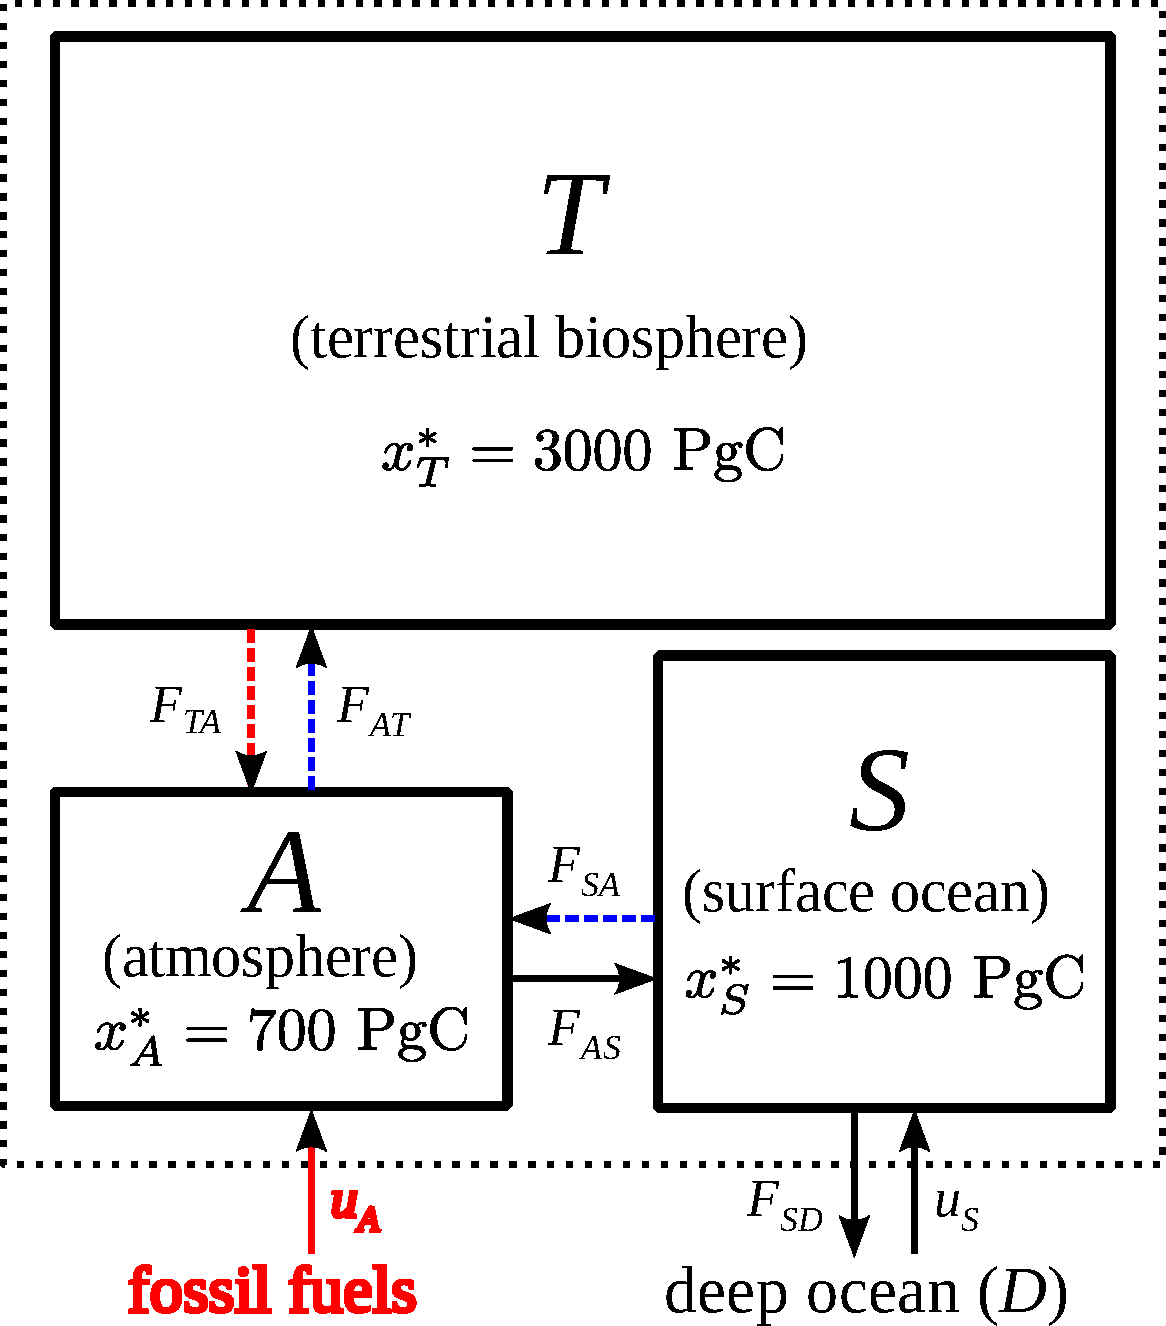
\includegraphics[width=0.9\lc,clip=true,trim= 0cm 0cm .5cm 0cm]{images/content/model.pdf}
	\end{column}
	\newlength{\rc}
	\setlength{\rc}{\the\dimexpr (\textwidth-\lc) \relax }
	\begin{column}{\rc}
		External input fluxes
		\begin{align*}
			&u_S = 45, \quad {\color{red}u_A(t)=\text{fossil-fuels}(t)}\\
			&\vspace{3.5cm}\\
			&F_{AT} = 60\,(x_A/700){\color{blue}^{0.2}}\\
			&F_{TA}(t) = 60\,x_T/3000\\
			&\qquad\qquad + {\color{red}\text{land-use-change}(t)}\\
			&F_{AS} = 100\,x_A/700\\
			&F_{SA} = 100\,(x_S/1000){\color{blue}^{10}}\\
			&\vspace{3.5cm}\\
			&F_{SD} = 45\,x_S/1000
		\end{align*}
	\end{column}
\end{columns}

		  \vspace{.5cm}	
	  }
	  %%%%%%%%%%%%%%%%%%%%%%%%%%%%%%%%%%%%%%%%%%%%%%%%%%%%%%%%%%%%%%%%%%%%%%%%%%%%%%
    % higher middle 
    \posterbox[title={Mathematical description}]{
      name=math,
      span=\leftspan,
      column=\leftcol,
      below =Overview 
    }{
	  	Well-mixed compartmental systems can be descibed by a system of generally \textbf{nonlinear} 
ordinary differential equations of the form
\vspace{-0.25cm}
\begin{equation}
	\deriv{t}\,\vec{x}(t) = \tens{A}(\vec{x}(t),t)\,\vec{x}(t)+\vec{u}(t),\quad t>t_0,
\end{equation}
%\vspace{-0.25cm}
with a given initial value $\vec{x_0}$.
\\
\vspace{1cm}
\\
{\Large Reduction to linear nonautonomous systems}
\\
\vspace{.5cm}
\\
\\
We assume to know (at least numerically) the unique solution of (1) and denote it by $\vec{x}$.
We then plug it into $\tens{A}(\vec{x},t))$ and obtain the {\bf linear} system of ordinarzy differential equations.
\[
\frac{d}{dt} \vec{x}(t) = \tens{A}(t)\vec{x}(t)+\vec{u}(t),\quad t>t_0
\]
This equation has the general solution formula
\[
	\vec{x}(t)=\underbrace{\tens{\Phi}(t,t_0)\vec{x}_0}_{\text{age}(t)=t-t_0+\text{initial age}}
	+ \int_{t_0}^t \underbrace{\tens{\Phi}(t,\tau)\vec{u}(\tau)}_{\text{age}(t)=t-\tau} d\tau,
\]
where $\tens{\Phi}$ is the so-called state transition matrix. This leads immediately to the 
\alert{vector of age densities} 
\[
\vec{\rho}(a,t)=
\begin{cases}
	\tens{\Phi}(t,t_0) \vec{\rho}_0(a-(t-t_0)),& a \ge t-t_0,
	\\
	\tens{\Phi}(t,t-a) \vec{u}(t-a),	& a < t-t_0,
\end{cases}
\]
where $\vec{\rho}_0$ is the initial age distribution.

		  \vspace{.5cm}	
	  }
	  %%%%%%%%%%%%%%%%%%%%%%%%%%%%%%%%%%%%%%%%%%%%%%%%%%%%%%%%%%%%%%%%%%%%%%%%%%%%%%
    % lower middle
    \posterbox[title={Pre-industrial (<1765), \\ system in steady state}]{
      name=preindustrial,
      span=\leftspan,
      column=\leftcol,
      between=math and Model
    }{
	  	\begin{columns}
	\setlength{\lc}{0.30\textwidth}
	\begin{column}{\lc}
		Transit time density
		
		$p_T(t) = \vec{z}^T\,e^{t\,\tens{A}}\,\vec{u}$
		\vspace{.5cm}	
		
		System age density
		
		$p_A(a) =\sum\limits_j \left(e^{a\,\tens{A}}\,\vec{u}\right)_j$
		\vspace{.5cm}	
		
		Compartmental \\
		age density

                $p_{j}(a) = \left(e^{a\,\tens{A}}\,\vec{u}\right)_j$
	\end{column}
	\setlength{\rc}{\the\dimexpr (\textwidth-\lc) \relax }
	\begin{column}{\rc}
		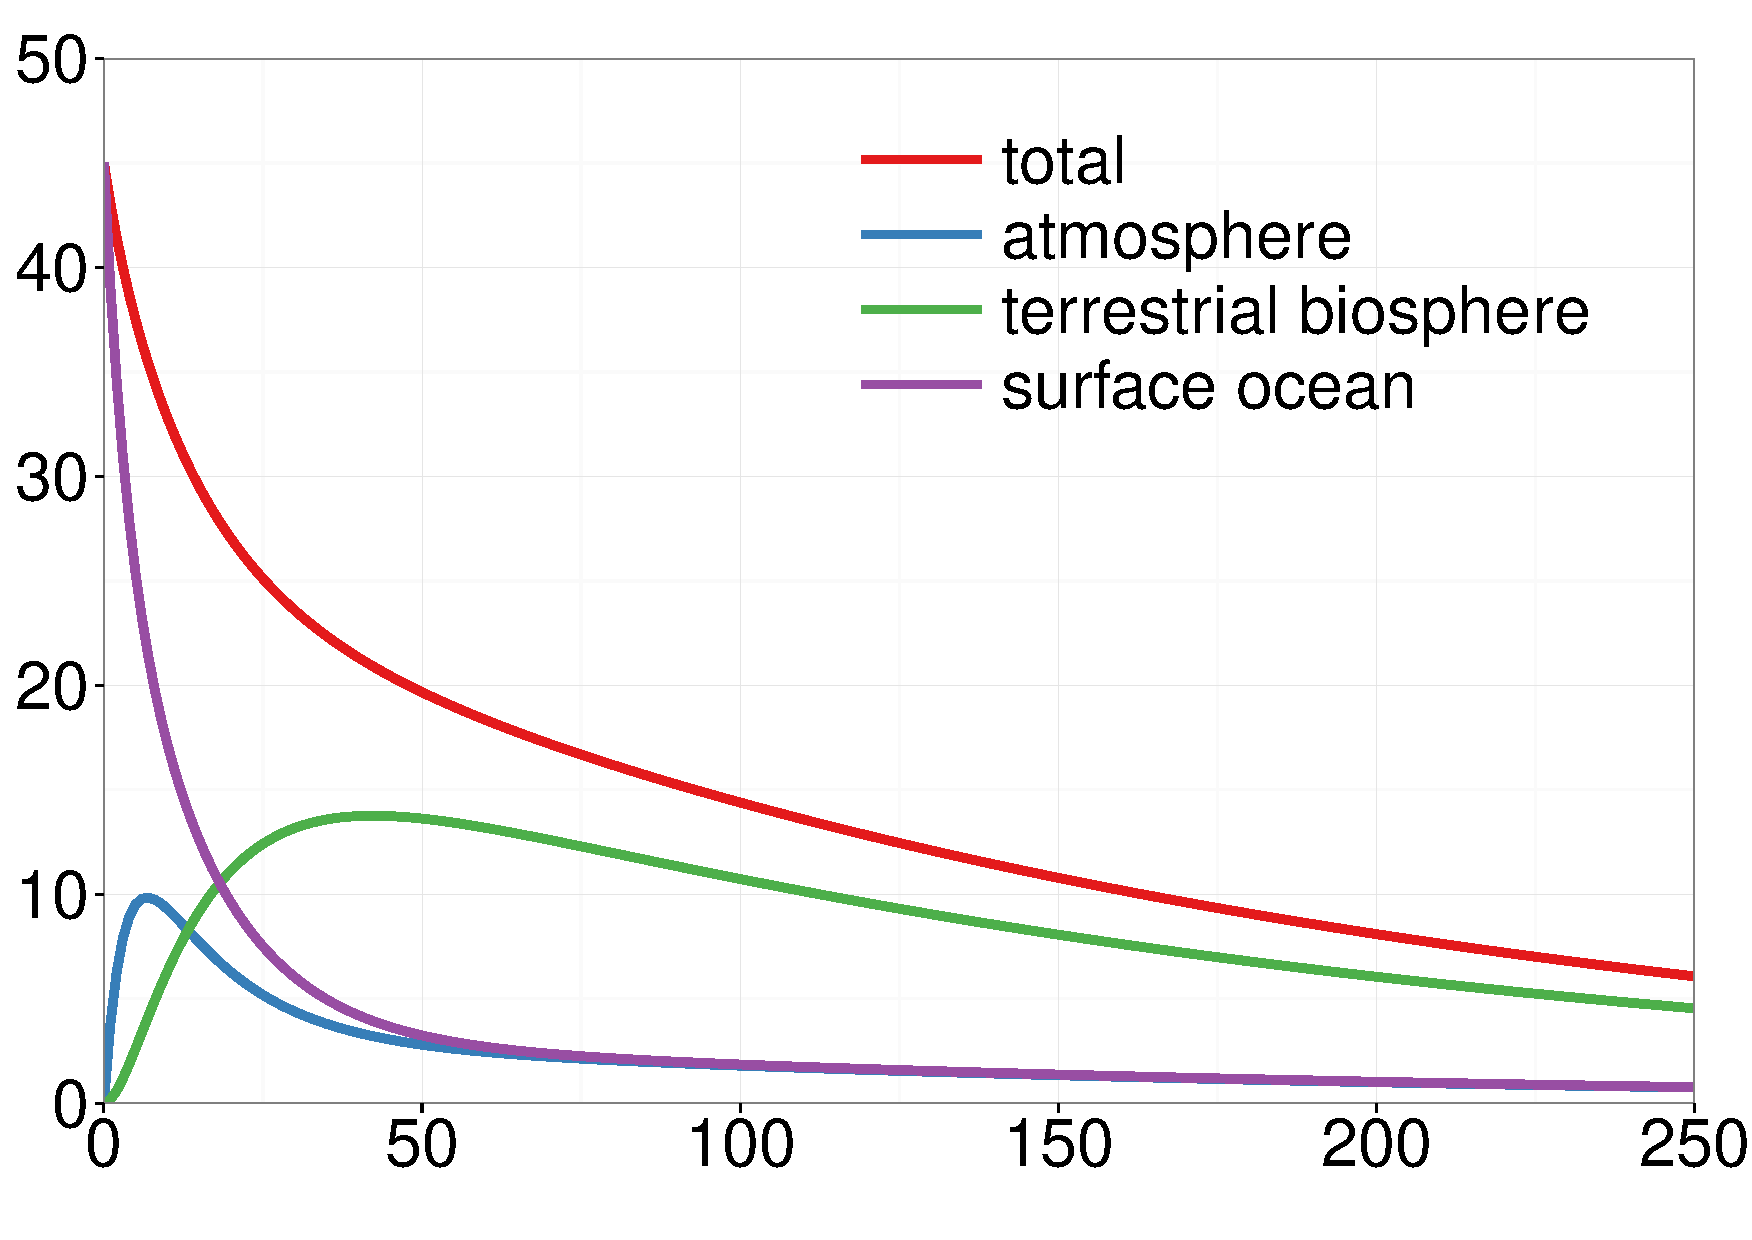
\includegraphics[width=0.9\rc]{images/content/ss.pdf}
	\end{column}
\end{columns}

	  }
  %%%%%%%%%%%%%%%%%%%%%%%%%%%%%%%%%%%%%%%%%%%%%%%%%%%%%%%%%%%%%%%%%%%%%%%%%%%%%%%
  % %second column  
    % top
      \posterbox[title= {State transition matrix}]{
        name=stateTransionMatrix, 
        column=\rightcol, 
        span= \rightspan
      }{
    	  \begin{center}
	\begin{tabular}{rll}
	one-dimensional & $\tens{\Phi}(t,t_0) = \exp\left[(t-t_0)\,A(t)\right]$ & exponential function\\
	
	multi-dimensional, & $\tens{\Phi}(t,t_0) = \exp\left[(t-t_0)\,A(t)\right]$ & matrix exponential \\
	autonomous\\
	
	multi-dimensional, & $ \frac{d}{dt} \tens{\Phi}(t,t_0)=\tens{A} \tens{\Phi}(t,t_0)$& only numerical\\
	nonautonomous && solution
	\end{tabular}
\end{center}

      }
    %%%%%%%%%%%%%%%%%%%%%%%%%%%%%%%%%%%%%%%%%%%%%%%%%%%%%%%%%%%%%%%%%%%%%%%%%%%%%%%
    % bottom 
    \posterbox[title=Bibliography] {
      name=bibliography,
      span=\rightspan,
      column=\rightcol, 
      above=bottom
    }{
      {
Anderson DH (1983) Compartmental modeling and tracer kinetics, vol 50. Springer Science \& Business Media \\
Manzoni S, Katul GG, Porporato A (2009) Analysis of soil carbon transit times and age distributions using network theories. 
    Journal of Geophysical Research 114(G4):1–14, DOI10.1029/2009JG001070 \\
Metzler H, Müller M, Sierra CA (2018) Age and transit time distributions of well-mixed compartmental systems, 
PNAS http://www.pnas.org/content/early/2018/01/19/1705296115.abstract\\
Metzler H, Sierra CA (2017) Mathematical Geosciences Linear autonomous compartmental models as continuous-time Markov chains: transit time and system age distributions \\
Rasmussen M, Hastings A, Smith MJ, Agusto FB, Chen-Charpentier BM, Hoffman FM, Jiang J, Todd-Brown KEO, Wang Y, 
Wang YP, Luo Y (2016) Transit times and mean ages for nonautonomous and autonomous compartmental systems. J Math Biol

      }
	  }
    %%%%%%%%%%%%%%%%%%%%%%%%%%%%%%%%%%%%%%%%%%%%%%%%%%%%%%%%%%%%%%%%%%%%%%%%%%%%%%
    % middle top
    \posterbox[title={ Perturbed (1765-2500)}]{
      name=Perturbed,
      span=\rightspan,
      column=\rightcol, 
      below=stateTransionMatrix 
    }{
    	\begin{columns}
	\setlength{\lc}{0.39\textwidth}
	\begin{column}{\lc}
		\begin{minipage}[T]{\textwidth}
			\centering{\large Anthropogenic perturbations}
			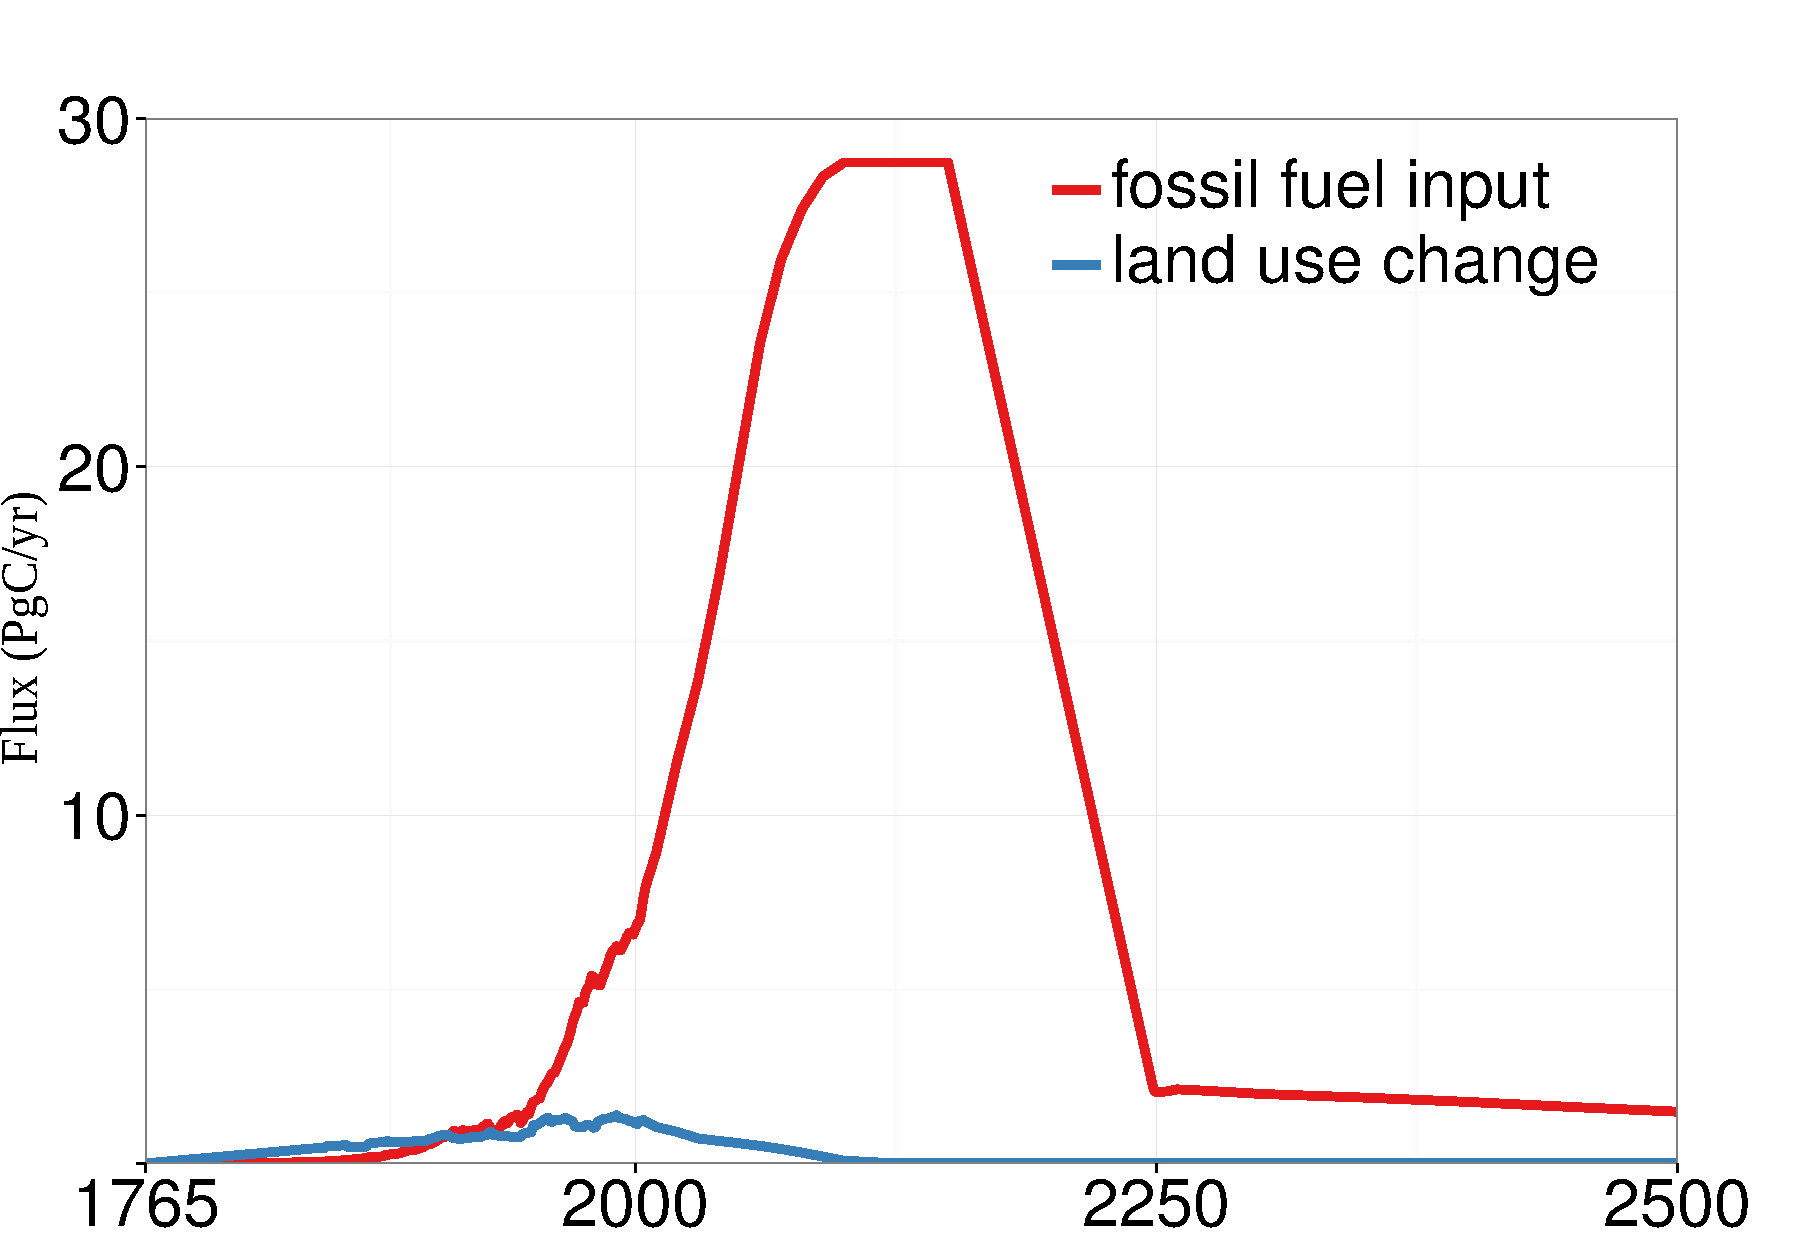
\includegraphics[width=0.9\lc]{images/content/ext_inp.pdf}
			\\
			\centering{\large Mean age and transit time}
			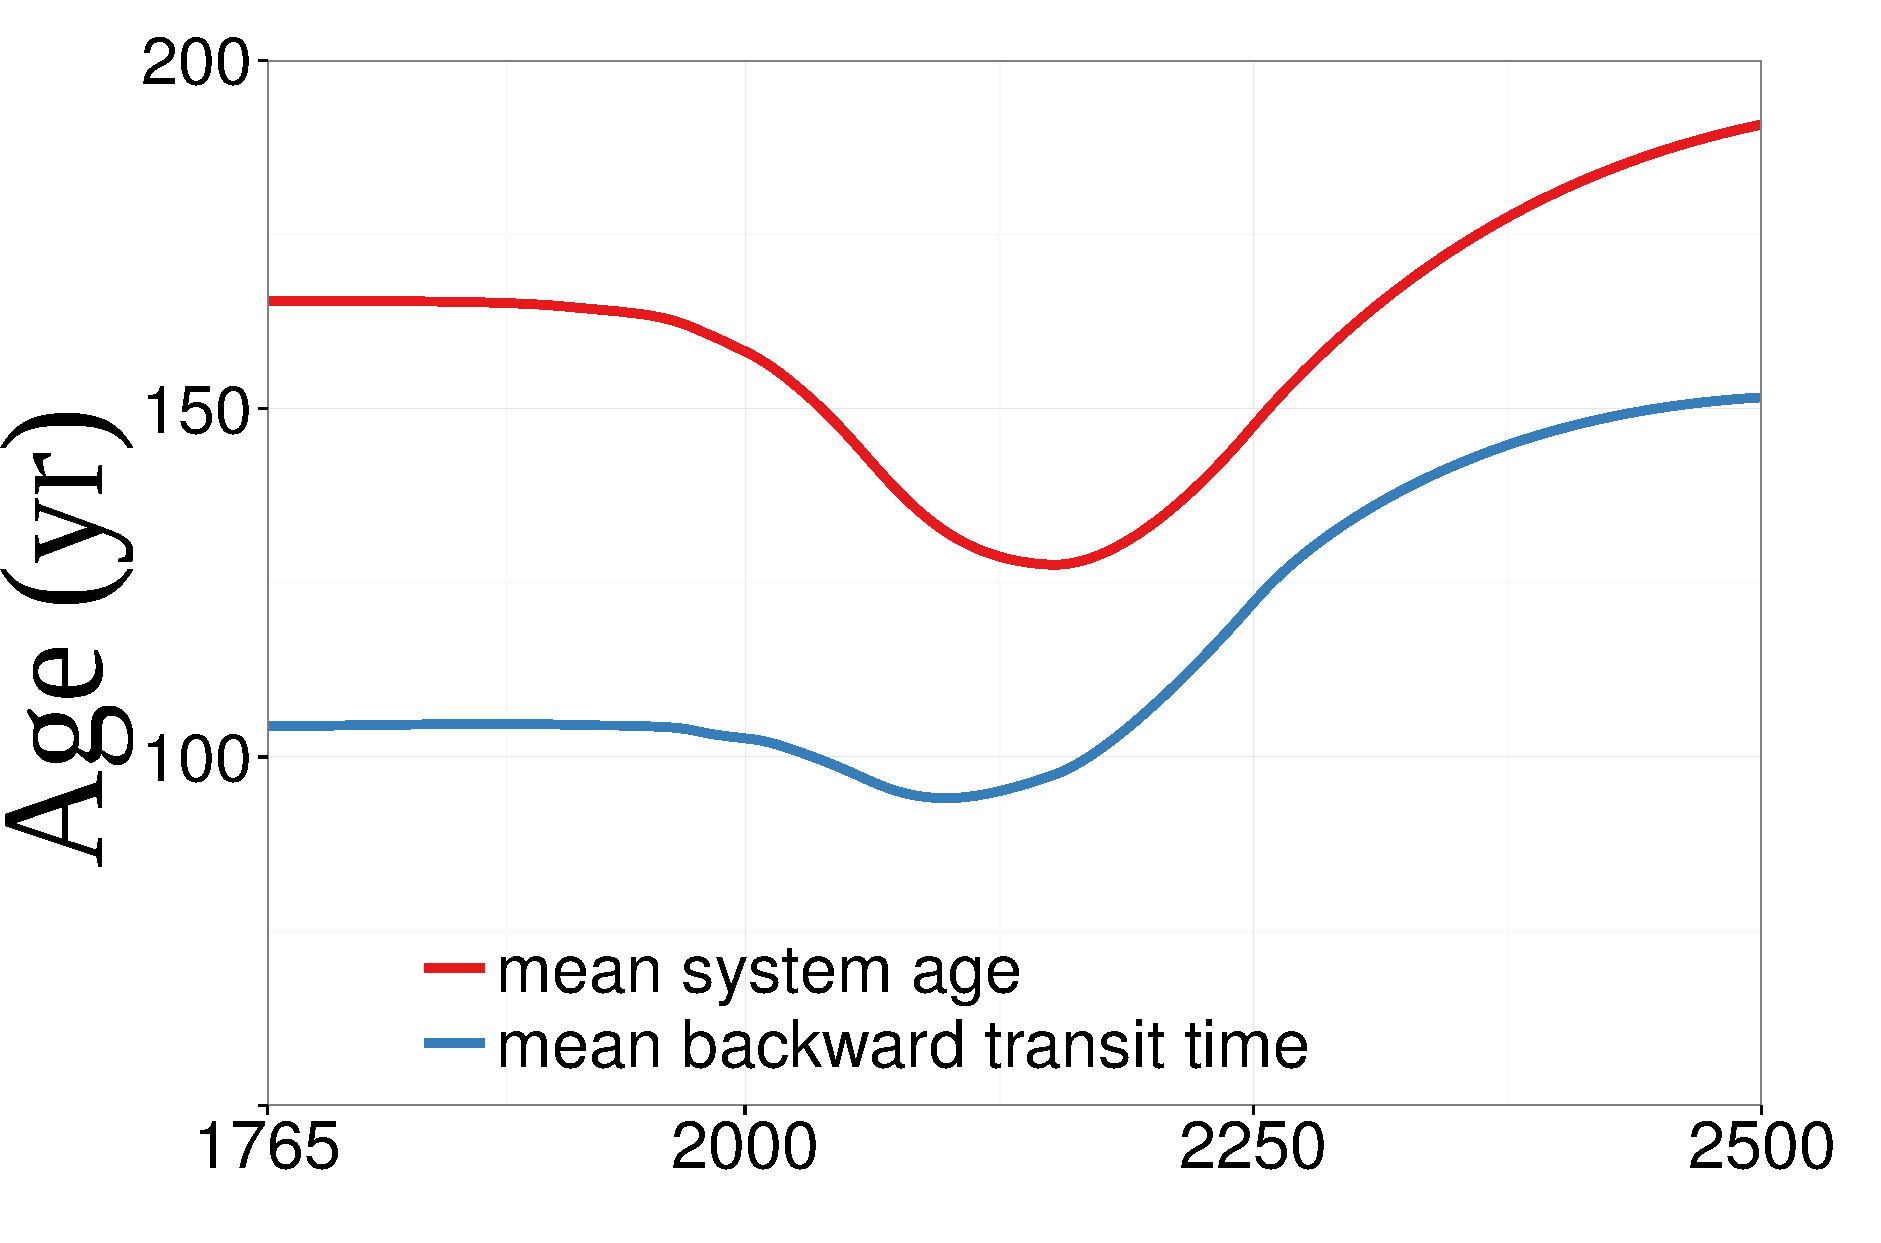
\includegraphics[width=0.9\lc]{images/content/means.pdf}
		\end{minipage}
	\end{column}
	\setlength{\rc}{\the\dimexpr (\textwidth-\lc) \relax }
	\begin{column}{\rc}
		\begin{minipage}[T]{\textwidth}
			\centering{\large Atmosphere}
			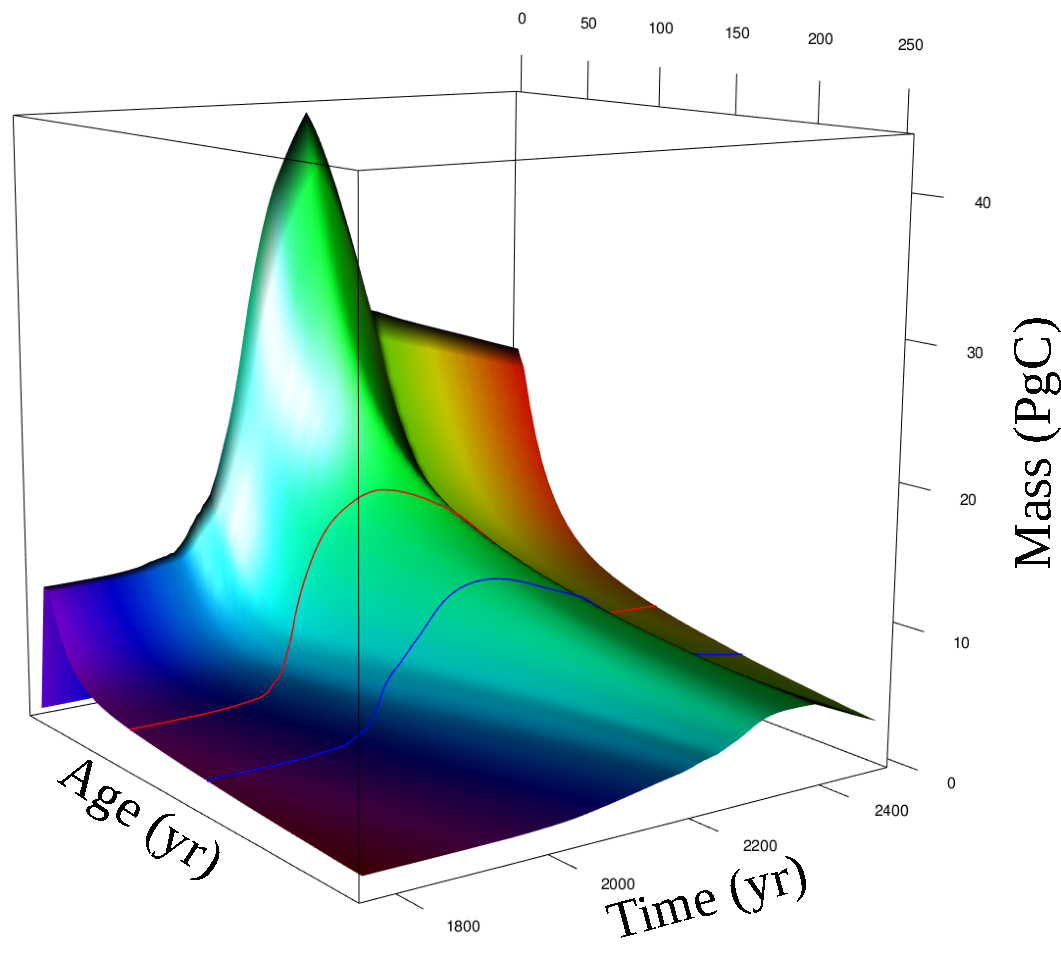
\includegraphics[width=0.9\rc]{images/content/3D.pdf}
		\end{minipage}
	\end{column}
\end{columns}

    }
    %%%%%%%%%%%%%%%%%%%%%%%%%%%%%%%%%%%%%%%%%%%%%%%%%%%%%%%%%%%%%%%%%%%%%%%%%%%%%%
    % middle 
    \posterbox[title={Transit time}]{
      name=TransitTime,
      span=\rightspan,
      column=\rightcol, 
      below=Perturbed 
    }{
    	If we define the (backward) transit time of a particle as the age of the particle 
at the time when it exits the system, we can easily derive explicit formulas for its distribution 
from the age distribution.\\
The simple approach stock/flux for the transit time is valid only for a system in steady state.
{\color{red}Out of steady state, stock($t$)/flux($t$) cannot be interpreted as a transit time.}


    }
    %%%%%%%%%%%%%%%%%%%%%%%%%%%%%%%%%%%%%%%%%%%%%%%%%%%%%%%%%%%%%%%%%%%%%%%%%%%%%%
    % middle 
    \posterbox[title={Forward Transit Time}]{
      name=Evolution,
      span=\rightspan,
      column=\rightcol, 
      below=TransitTime 
    }{
    	% vim:set ff=unix expandtab ts=2 sw=2:
\begin{columns}
	\setlength{\lc}{0.5\textwidth}
	\begin{column}{\lc}
	  \begin{center}
      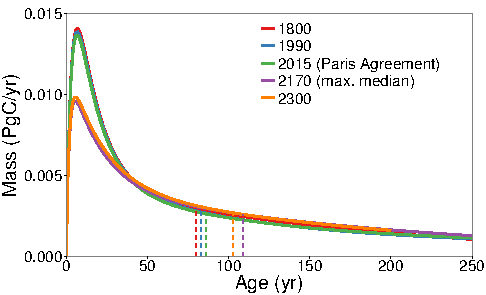
\includegraphics[width=\linewidth]{images/content/ftt.pdf}
	  \end{center}
	\end{column}
	\setlength{\rc}{\the\dimexpr (\textwidth-\lc) \relax }
	\begin{column}{\rc}
    \begin{minipage}{0.95\rc}
    Forward transit-time densities of $1\, \text{PgC}$ %$1\, \si{\peta\gram\carbon}$ 
      hypothetically injected into the atmosphere in the years 1800 (red), 1990 (blue), 2015 (green), 2170 (purple), and 2300 (orange).
      The orange curve ends at the age of 200, because our simulation only lasts until the year 2500.
      The medians (dashed vertical lines) increase until the year 2170 and then start decreasing.
      \label{fig:ftt}
    \end{minipage}
	\end{column}
\end{columns}

    }
    %%%%%%%%%%%%%%%%%%%%%%%%%%%%%%%%%%%%%%%%%%%%%%%%%%%%%%%%%%%%%%%%%%%%%%%%%%%%%%
    % middle bottom
    \posterbox[title={Classification}]{
      name=Classification,
      span=\rightspan,
      column=\rightcol, 
      between=Evolution and bibliography
    }{
    	\begin{columns}
	\setlength{\lc}{0.5\textwidth}
	\begin{column}{\lc}
	\begin{center}
		\begin{tabular}{rl}
		 $\tens{A}(\vec{x}(t), t)$ & nonlinear, \\
		 $\tens{A}(\vec{x}(t)), \vec{u}(t)$ & nonautonomous\\
		 \hline
		 $\tens{A}(\vec{x}(t)), \vec{u}$ & nonlinear,\\
		& autonomous \\
		 \hline
		 $\tens{A}(t), \vec{u}$ & linear, \\
		 $\tens{A}, \vec{u}(t)$ & nonautonomous\\
		 $\tens{A}(t), \vec{u}(t)$\\
		 \hline
		 $\tens{A}, \vec{u}$ & linear,\\
		&  autonomous
		\end{tabular}
	\end{center}
	\end{column}
	\setlength{\rc}{\the\dimexpr (\textwidth-\lc) \relax }
	\begin{column}{\rc}
		\begin{center}
		\begin{tabular}{rl}
		  $\vec{x}(t)$ & vector of compartment \\
		& content (e.g. C) at time $t$\\
		  $\tens{A}$ & compartmental matrix,\\
		 & describes fluxes between\\
		 & compartments\\
		  $\vec{z}(t)$ & external outflux vector\\
		 &  at time $t$\\
		  $\vec{u}(t)$ & external input vector\\
		 & at time $t$\\
		\end{tabular}
	\end{center}
	\end{column}
\end{columns}

    }
\end{tcbposter}
	
  
  \end{frame}
\end{document}

          \bibliography{GeneralModel} % for an extra page
          \bibliographystyle{abbrvnat}
        \end{multicols}
      }
	  }
    %%%%%%%%%%%%%%%%%%%%%%%%%%%%%%%%%%%%%%%%%%%%%%%%%%%%%%%%%%%%%%%%%%%%%%%%%%%%%%
    % middle
    \posterbox[title={ Conclusion }]{
      name=Intro,
      span=\rightspan,
      column=\rightcol, 
      between=combi and bibliography
    }{
    	
% vim:set ff=unix expandtab ts=2 sw=2:
%%%%%%%%%%%%%%%%%%%%%%%%%%%%%%%%%%%%%%%%%%%%%%%%%%%%%%%%%%%%%%%%%%%%%%%%%%%%%%
\noindent
\begin{itemize}
  \item
  Autonomous concepts like steady state are clearly insufficient for the analysis of non-autonomous systems.
  \item 
  Nonautonomous techniques are often restricted to linear systems.
  \item
  We propose Input to State Stability (ISS) as
  candidate for the necessary generalization of the established analysis with
  respect to equilibria or invariant sets for autonomous systems, 
  \item 
  In the just puplished  paper \cite{MuellerSierra2017TE} 
  we showed: 
  \begin{itemize}
  \item 
    How ISS generalizes existent concepts formerly only available for Linear Time Invariant (LTI) 
  and Linear Time Variant (LTV) systems to the nonlinear case. 
  \item 
    Exmaples applying it to reservoir models typical for element cycling in
  ecosystem, e.g. in soil organic matter decomposition.  
  \end{itemize}
\end{itemize}

    }

\end{tcbposter}
